\chapter{Architecture Design}

\section{Architectural Diagram}

\begin{figure}[H]
    \centering
    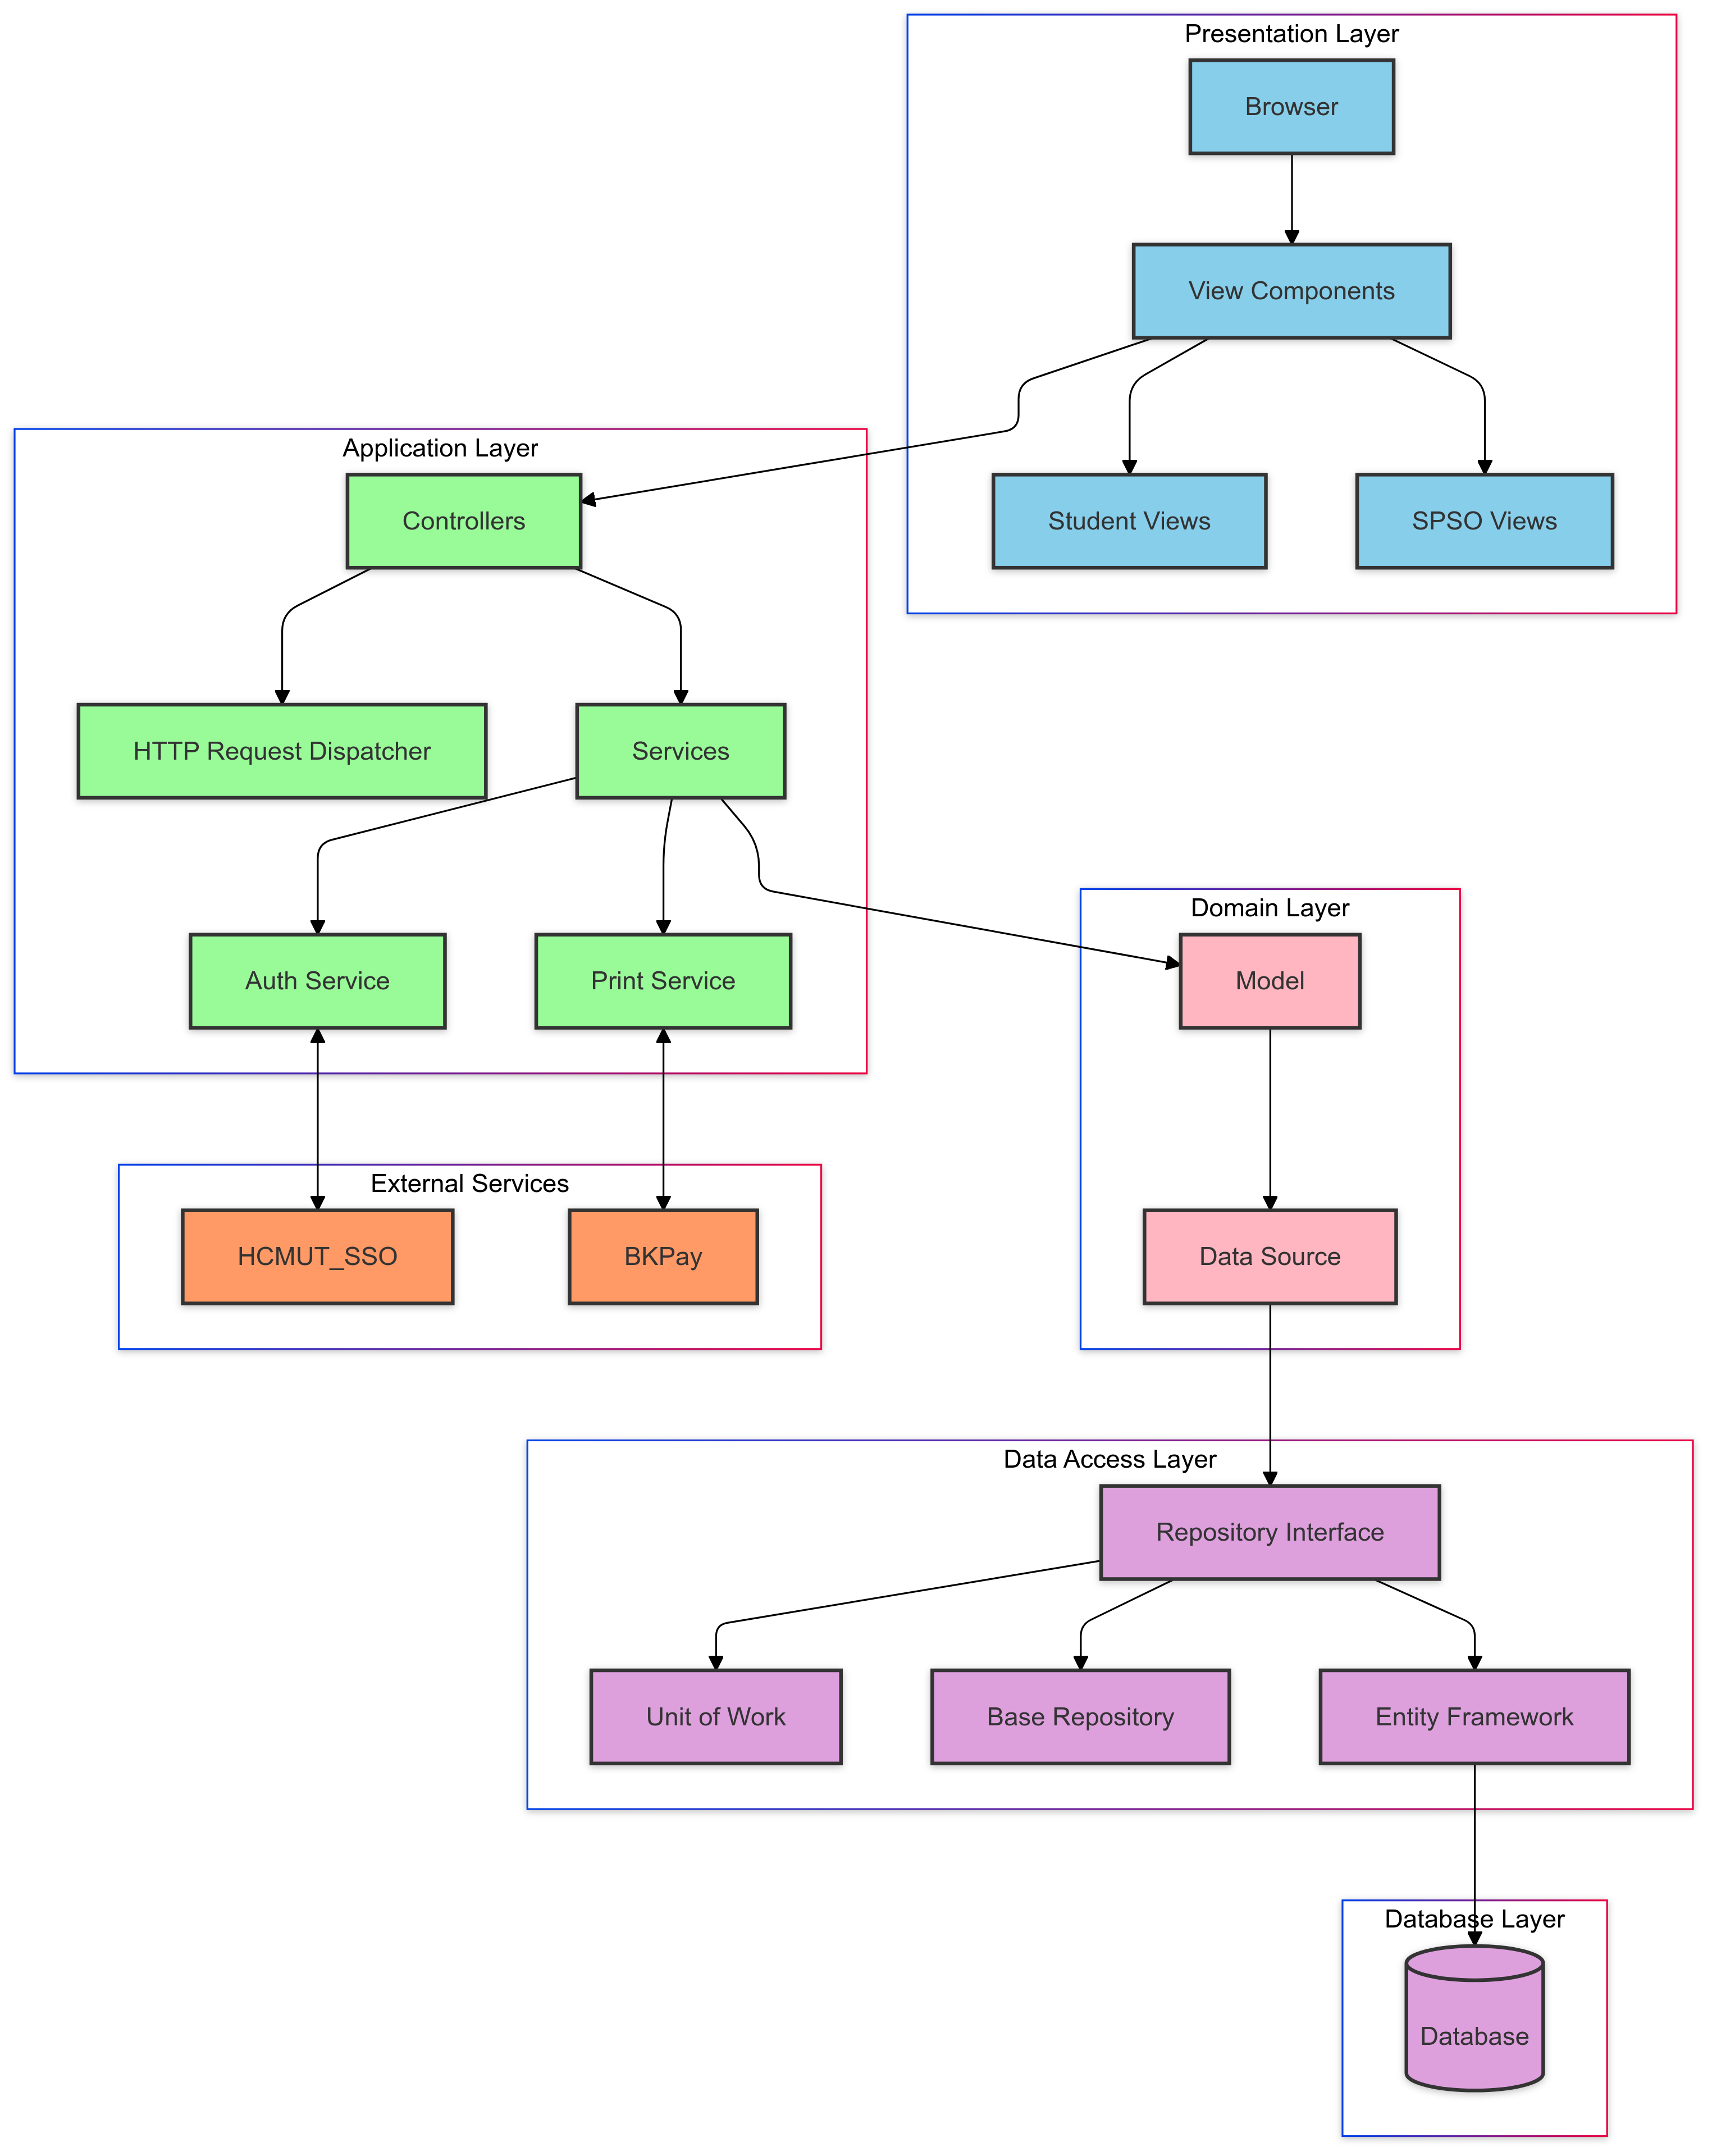
\includegraphics[width=0.78\linewidth]{images/architectural_diagram.png}
    \caption{Architectural Diagram}
    \label{fig:enter-label}
\end{figure}

\subsection{Presentation Strategy} 

The HCMUT-SSPS system implements a client-side architecture focusing on separation of concerns between UI components and business logic. We adopt a component-based architecture to promote reusability and maintainability across different views (student and SPSO interfaces). The presentation layer implements the Observer pattern for state management, ensuring consistent data flow and real-time updates for printing statuses. For optimal performance, we utilize lazy loading for resource-heavy components and implement efficient client-side caching mechanisms. The UI follows a responsive design approach with mobile-first principles, ensuring accessibility across different devices and screen sizes.

\subsection{Data Storage Approach} 

Our data persistence strategy implements a layered approach with clear separation between data access and business logic. The system utilizes a relational database for structured data (user profiles, transactions, print logs) with a document store for handling print job files and documents. We implement the Repository pattern to abstract data access operations, coupled with Unit of Work pattern for maintaining data consistency across transactions. The storage layer includes caching mechanisms for frequently accessed data and implements database sharding for horizontal scalability. This architecture supports our requirements for data integrity, performance, and scalability while maintaining ACID compliance for critical transactions.

\subsection{API Management} 

The API architecture follows RESTful principles with clear resource-oriented endpoints and standardized response formats. We implement an API Gateway pattern for request routing, composition, and protocol translation. Authentication is integrated with HCMUT's SSO system, while authorization implements role-based access control (RBAC). The API layer includes the following;

\begin{multicols}{2}    
\begin{itemize}
    \item Request validation and sanitization
    \item Rate limiting and throttling
    \item Standardized error handling
    \item API versioning through URL paths
    \item Response compression and caching
    \item Monitoring and logging capabilities
\end{itemize}
\end{multicols}

\subsection{Key Architectural Principles}

\subsubsection{Separation of Concerns}
\begin{itemize}
    \item Clear boundaries between presentation, business logic, and data access
    \item Modular components for easy maintenance and testing
    \item Standardized interfaces between layers
\end{itemize}

\begin{multicols}{2}
\subsubsection{Scalability}
\begin{itemize}
    \item Horizontal scaling capabilities
    \item Efficient caching strategies
    \item Load balancing support
\end{itemize}

\subsubsection{Security}
\begin{itemize}
    \item Integration with institutional SSO
    \item Secure data transmission
    \item Input validation and sanitization
    \item Access control and audit logging
\end{itemize}

\subsubsection{Maintainability}
\begin{itemize}
    \item Documented API contracts
    \item Clear coding standards
    \item Version control strategies
    \item Comprehensive logging
\end{itemize}

\subsubsection{Performance}
\begin{itemize}
    \item Optimized database queries
    \item Client-side caching
    \item Resource optimization
    \item Response compression
\end{itemize}
\end{multicols}

\newpage
\section{Component Diagram}
\subsection{Component Diagram Design}
\begin{figure}[H]
    \centering
    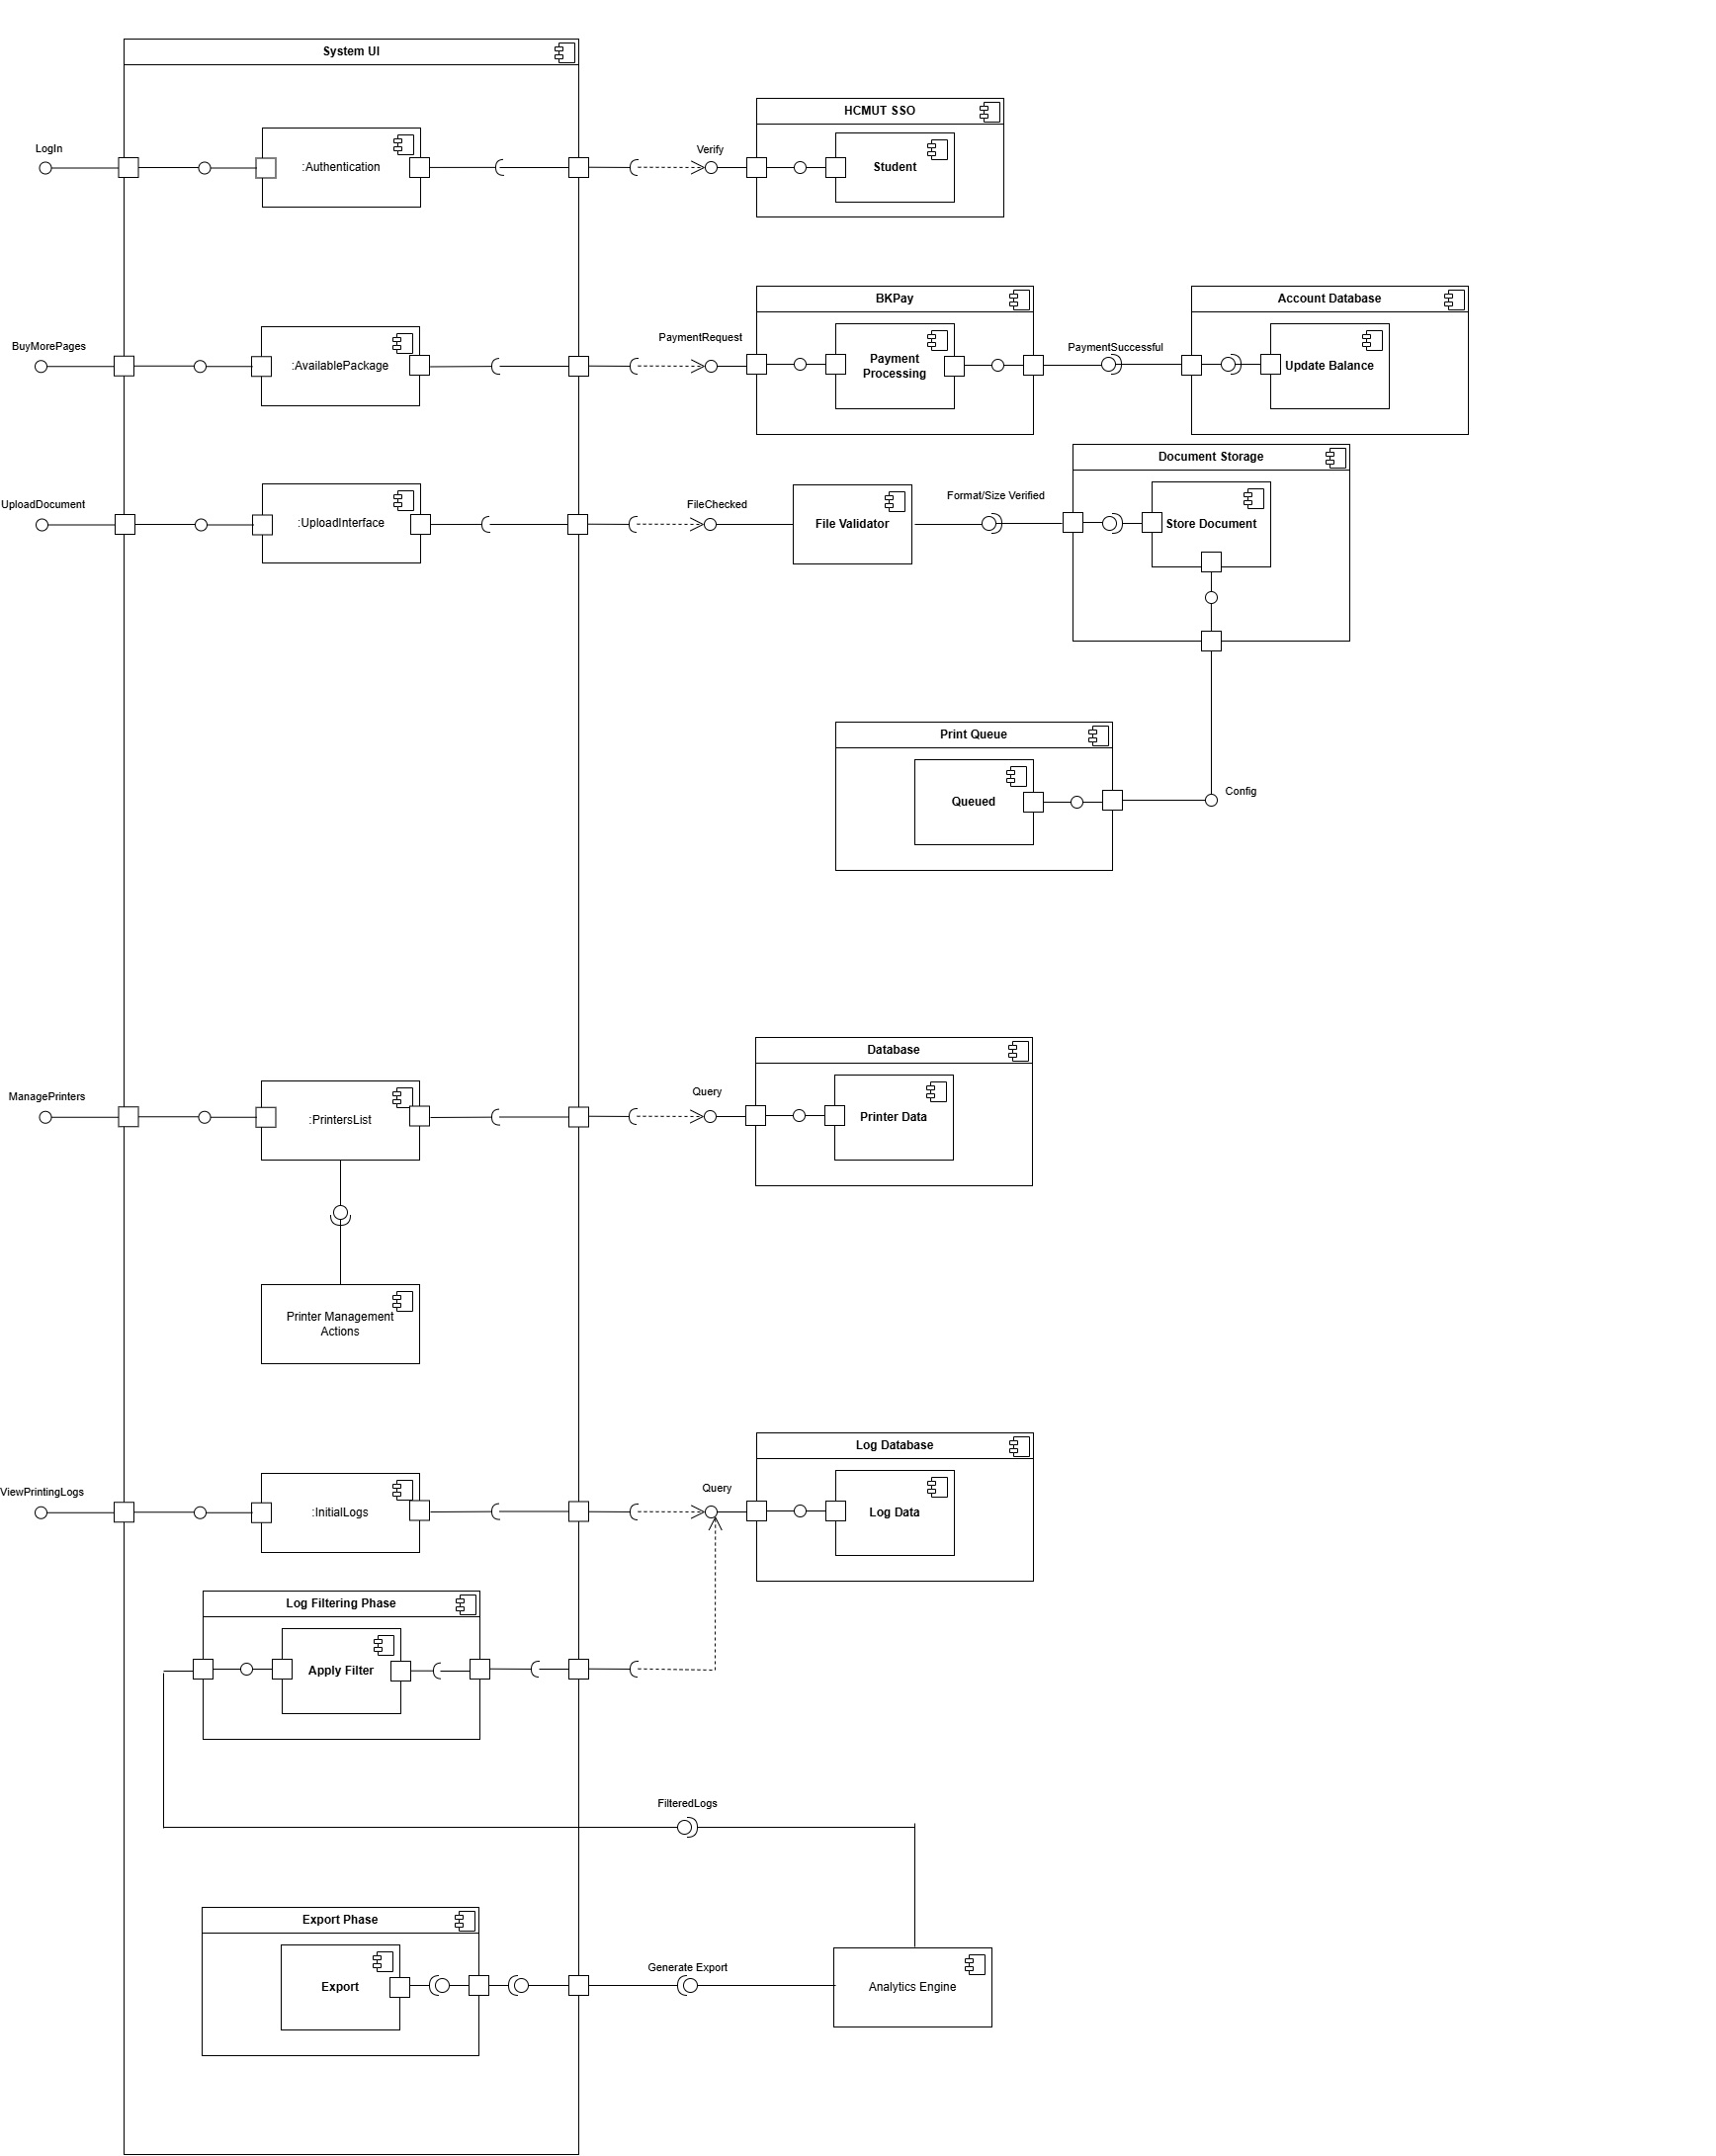
\includegraphics[width=1\linewidth]{images/component_diagram.png}
    \caption{Component Diagram}
    \label{fig:enter-label}
\end{figure}

\newpage
\subsection{Description}
The component diagram highlights the major components and their interactions with each other to fulfill the system’s functionality.
\begin{enumerate}
    \item  The “LogIn” diagram handles user authentication which interacts with the “HCMUT SSO” to verify user credentials and the System UI to provide a user interface for login.
    \item The “BuyMorePages” diagram give user choice of package to buy, which interacts with “BKPay” for Students to pay for the chosen and the System UI to provide a user interface for the service. The “Account Database” will interact with the “BKPay” as long as the payment is successful.
    \item The “UploadDocument” diagram interacts with the System UI to provide a user interface to upload the user document and interacts with the “File Validator” to have the file’s format and size checked. Since the uploaded files meet the required specifications, they are stored in the Document Storage and also queued for printing after print setting configuration.
    \item The “ManagePrinters” diagram provide the user interface where users can view and manage printers. The PrinterList queries the “Database” to manage printers and printers data. The “Printers Management Actions” start its implementation when users perform printers management actions, querying “Database” for printers data.
    \item The “ViewPrintingLogs” diagram provides the user interface where users can view and interact with the logs, the System querying the “Log Database” for the log data. After user applying specific filter. The “Log Filtering Phase” queries the “Log Database” for the requested filtered data and show them for users. In the “Export Phase”, the system processes the user’s request and generates a report through the Analytics Engine, the engine get the filtered logs data from the “Log Filtered Phase”. The generated report is then made available for users to download.
\end{enumerate}

\newpage